% Options for packages loaded elsewhere
\PassOptionsToPackage{unicode}{hyperref}
\PassOptionsToPackage{hyphens}{url}
%
\documentclass[
]{book}
\usepackage{amsmath,amssymb}
\usepackage{lmodern}
\usepackage{iftex}
\ifPDFTeX
  \usepackage[T1]{fontenc}
  \usepackage[utf8]{inputenc}
  \usepackage{textcomp} % provide euro and other symbols
\else % if luatex or xetex
  \usepackage{unicode-math}
  \defaultfontfeatures{Scale=MatchLowercase}
  \defaultfontfeatures[\rmfamily]{Ligatures=TeX,Scale=1}
\fi
% Use upquote if available, for straight quotes in verbatim environments
\IfFileExists{upquote.sty}{\usepackage{upquote}}{}
\IfFileExists{microtype.sty}{% use microtype if available
  \usepackage[]{microtype}
  \UseMicrotypeSet[protrusion]{basicmath} % disable protrusion for tt fonts
}{}
\makeatletter
\@ifundefined{KOMAClassName}{% if non-KOMA class
  \IfFileExists{parskip.sty}{%
    \usepackage{parskip}
  }{% else
    \setlength{\parindent}{0pt}
    \setlength{\parskip}{6pt plus 2pt minus 1pt}}
}{% if KOMA class
  \KOMAoptions{parskip=half}}
\makeatother
\usepackage{xcolor}
\usepackage{color}
\usepackage{fancyvrb}
\newcommand{\VerbBar}{|}
\newcommand{\VERB}{\Verb[commandchars=\\\{\}]}
\DefineVerbatimEnvironment{Highlighting}{Verbatim}{commandchars=\\\{\}}
% Add ',fontsize=\small' for more characters per line
\usepackage{framed}
\definecolor{shadecolor}{RGB}{248,248,248}
\newenvironment{Shaded}{\begin{snugshade}}{\end{snugshade}}
\newcommand{\AlertTok}[1]{\textcolor[rgb]{0.94,0.16,0.16}{#1}}
\newcommand{\AnnotationTok}[1]{\textcolor[rgb]{0.56,0.35,0.01}{\textbf{\textit{#1}}}}
\newcommand{\AttributeTok}[1]{\textcolor[rgb]{0.77,0.63,0.00}{#1}}
\newcommand{\BaseNTok}[1]{\textcolor[rgb]{0.00,0.00,0.81}{#1}}
\newcommand{\BuiltInTok}[1]{#1}
\newcommand{\CharTok}[1]{\textcolor[rgb]{0.31,0.60,0.02}{#1}}
\newcommand{\CommentTok}[1]{\textcolor[rgb]{0.56,0.35,0.01}{\textit{#1}}}
\newcommand{\CommentVarTok}[1]{\textcolor[rgb]{0.56,0.35,0.01}{\textbf{\textit{#1}}}}
\newcommand{\ConstantTok}[1]{\textcolor[rgb]{0.00,0.00,0.00}{#1}}
\newcommand{\ControlFlowTok}[1]{\textcolor[rgb]{0.13,0.29,0.53}{\textbf{#1}}}
\newcommand{\DataTypeTok}[1]{\textcolor[rgb]{0.13,0.29,0.53}{#1}}
\newcommand{\DecValTok}[1]{\textcolor[rgb]{0.00,0.00,0.81}{#1}}
\newcommand{\DocumentationTok}[1]{\textcolor[rgb]{0.56,0.35,0.01}{\textbf{\textit{#1}}}}
\newcommand{\ErrorTok}[1]{\textcolor[rgb]{0.64,0.00,0.00}{\textbf{#1}}}
\newcommand{\ExtensionTok}[1]{#1}
\newcommand{\FloatTok}[1]{\textcolor[rgb]{0.00,0.00,0.81}{#1}}
\newcommand{\FunctionTok}[1]{\textcolor[rgb]{0.00,0.00,0.00}{#1}}
\newcommand{\ImportTok}[1]{#1}
\newcommand{\InformationTok}[1]{\textcolor[rgb]{0.56,0.35,0.01}{\textbf{\textit{#1}}}}
\newcommand{\KeywordTok}[1]{\textcolor[rgb]{0.13,0.29,0.53}{\textbf{#1}}}
\newcommand{\NormalTok}[1]{#1}
\newcommand{\OperatorTok}[1]{\textcolor[rgb]{0.81,0.36,0.00}{\textbf{#1}}}
\newcommand{\OtherTok}[1]{\textcolor[rgb]{0.56,0.35,0.01}{#1}}
\newcommand{\PreprocessorTok}[1]{\textcolor[rgb]{0.56,0.35,0.01}{\textit{#1}}}
\newcommand{\RegionMarkerTok}[1]{#1}
\newcommand{\SpecialCharTok}[1]{\textcolor[rgb]{0.00,0.00,0.00}{#1}}
\newcommand{\SpecialStringTok}[1]{\textcolor[rgb]{0.31,0.60,0.02}{#1}}
\newcommand{\StringTok}[1]{\textcolor[rgb]{0.31,0.60,0.02}{#1}}
\newcommand{\VariableTok}[1]{\textcolor[rgb]{0.00,0.00,0.00}{#1}}
\newcommand{\VerbatimStringTok}[1]{\textcolor[rgb]{0.31,0.60,0.02}{#1}}
\newcommand{\WarningTok}[1]{\textcolor[rgb]{0.56,0.35,0.01}{\textbf{\textit{#1}}}}
\usepackage{longtable,booktabs,array}
\usepackage{calc} % for calculating minipage widths
% Correct order of tables after \paragraph or \subparagraph
\usepackage{etoolbox}
\makeatletter
\patchcmd\longtable{\par}{\if@noskipsec\mbox{}\fi\par}{}{}
\makeatother
% Allow footnotes in longtable head/foot
\IfFileExists{footnotehyper.sty}{\usepackage{footnotehyper}}{\usepackage{footnote}}
\makesavenoteenv{longtable}
\usepackage{graphicx}
\makeatletter
\def\maxwidth{\ifdim\Gin@nat@width>\linewidth\linewidth\else\Gin@nat@width\fi}
\def\maxheight{\ifdim\Gin@nat@height>\textheight\textheight\else\Gin@nat@height\fi}
\makeatother
% Scale images if necessary, so that they will not overflow the page
% margins by default, and it is still possible to overwrite the defaults
% using explicit options in \includegraphics[width, height, ...]{}
\setkeys{Gin}{width=\maxwidth,height=\maxheight,keepaspectratio}
% Set default figure placement to htbp
\makeatletter
\def\fps@figure{htbp}
\makeatother
\setlength{\emergencystretch}{3em} % prevent overfull lines
\providecommand{\tightlist}{%
  \setlength{\itemsep}{0pt}\setlength{\parskip}{0pt}}
\setcounter{secnumdepth}{5}
\usepackage{booktabs}
\ifLuaTeX
  \usepackage{selnolig}  % disable illegal ligatures
\fi
\usepackage[]{natbib}
\bibliographystyle{plainnat}
\IfFileExists{bookmark.sty}{\usepackage{bookmark}}{\usepackage{hyperref}}
\IfFileExists{xurl.sty}{\usepackage{xurl}}{} % add URL line breaks if available
\urlstyle{same} % disable monospaced font for URLs
\hypersetup{
  pdftitle={Jenny's Stats Journey},
  pdfauthor={Jenny Sloane},
  hidelinks,
  pdfcreator={LaTeX via pandoc}}

\title{Jenny's Stats Journey}
\author{Jenny Sloane}
\date{2023-06-17}

\begin{document}
\maketitle

{
\setcounter{tocdepth}{1}
\tableofcontents
}
\hypertarget{about}{%
\chapter{About}\label{about}}

This is compilation of my notes from different topics in statistics. Each chapter covers a different topic. Resources and references are included.

\hypertarget{linear-regression}{%
\chapter{Linear Regression}\label{linear-regression}}

Primary reference for this chapter: \href{https://www.youtube.com/playlist?list=PLQGe6zcSJT0V4xC1NDyQePkyxUj8LWLnD}{Center Stat: Linear Regression Tutorials}.

\hypertarget{intro-to-linear-regression}{%
\section{Intro to Linear Regression}\label{intro-to-linear-regression}}

Linear regression is the foundation for more advanced techniques like structural equation model, factor analysis, multi level models, mixed effect models, etc. We are interested in exploring the statistical relationship: we are predicting outcomes (not a deterministic relationship).

Uses example with experience and performance where our outcome measure is \textbf{experience (x)} and our predictor is \textbf{performance (y)}. We can build a model to see how the average level of performance changes as a function of experience.

In a regression model we have:

\[
Yi = f(x) + \epsilon
\]

\begin{itemize}
\tightlist
\item
  A function to characterize the relationship between x and y
\item
  And there is also an inherent randomness for any individual represented by \(\epsilon\)
\end{itemize}

Of course a linear regression model is linear\ldots{} so the function is a straight line.

What everyone learned in school:

\[
Y = mx + b
\]

\begin{itemize}
\tightlist
\item
  where m is the slope of the line and b is the intercept
\end{itemize}

More formally:

\[
Yi = \beta_0 + \beta_1x_i  + \epsilon_i
\]
3 parameters of interest (assuming 1 predictor model)

\begin{enumerate}
\def\labelenumi{\arabic{enumi}.}
\tightlist
\item
  \(\beta_0\)
\end{enumerate}

\begin{itemize}
\tightlist
\item
  This is the intercept, which can be interpreted as the expected value of y when x = 0.
\item
  Note: sometimes the intercept can be meaningless.
\end{itemize}

\begin{enumerate}
\def\labelenumi{\arabic{enumi}.}
\setcounter{enumi}{1}
\tightlist
\item
  \(\beta_1\)
\end{enumerate}

\begin{itemize}
\tightlist
\item
  Change in y for a 1 unit change in x. Also known as the rise over run. How much change do we expect to change in our outcome given a 1 unit change in our predictor?
\end{itemize}

\begin{enumerate}
\def\labelenumi{\arabic{enumi}.}
\setcounter{enumi}{2}
\tightlist
\item
  \(\sigma^2\)
\end{enumerate}

\begin{itemize}
\tightlist
\item
  Variance of residuals
\end{itemize}

\hypertarget{demo}{%
\section{Demo}\label{demo}}

I made a fake crossfit dataset for this demo:

\begin{itemize}
\tightlist
\item
  \texttt{weight} = weight in pounds
\item
  \texttt{classes} = total number of crossfit classes attended
\item
  \texttt{clean\_weight} = one of the olympic weight movements in crossfit is called cleans. This variable is the max weight in pounds for each individual
\item
  \texttt{mile1} = time in minutes to complete mile 1
\item
  \texttt{mile2} = time in minutes to complete mile 2
\end{itemize}

\begin{verbatim}
## # A tibble: 6 x 7
##      id sex    weight classes clean_weight mile1 mile2
##   <dbl> <chr>   <dbl>   <dbl>        <dbl> <dbl> <dbl>
## 1     1 female    125      15           65   8.7   9.9
## 2     2 female    138      45          150  10.3  10.5
## 3     3 female    108       3           35  12.3  12.9
## 4     4 male      177      22          250   7.3   7  
## 5     5 male      190       8          150  10.7  11.2
## 6     6 female    186      77          170  10.2  10.5
\end{verbatim}

Let's plot the relationship between classes and cleans. We may predict that the number of classes people attend may positively correlate with clean weight

Of course, we may expect sex to influence our results, but we'll ignore that for now.

\begin{Shaded}
\begin{Highlighting}[]
\FunctionTok{ggplot}\NormalTok{(mydat, }\FunctionTok{aes}\NormalTok{(}\AttributeTok{x=}\NormalTok{classes, }\AttributeTok{y=}\NormalTok{clean\_weight)) }\SpecialCharTok{+}
  \FunctionTok{geom\_point}\NormalTok{() }\SpecialCharTok{+}
  \FunctionTok{theme\_bw}\NormalTok{() }\SpecialCharTok{+}
  \FunctionTok{labs}\NormalTok{(}\AttributeTok{x =} \StringTok{"Number of Classes"}\NormalTok{, }\AttributeTok{y =} \StringTok{"Clean Weight (pounds)"}\NormalTok{)}
\end{Highlighting}
\end{Shaded}

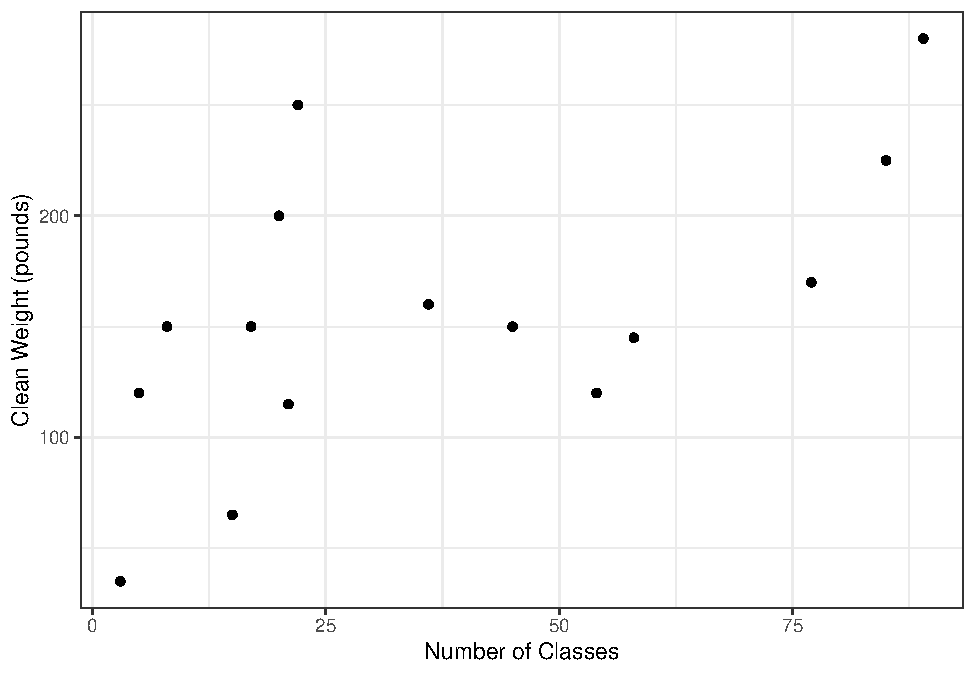
\includegraphics{_main_files/figure-latex/unnamed-chunk-2-1.pdf}

It looks like there's a positive relationship. Let's add in a regression line or line of best fit.

Using the \texttt{ggpubr} package, we can add the correlation coefficient (and p-value) along with the regression line equation.

\begin{Shaded}
\begin{Highlighting}[]
\FunctionTok{ggplot}\NormalTok{(mydat, }\FunctionTok{aes}\NormalTok{(}\AttributeTok{x=}\NormalTok{classes, }\AttributeTok{y=}\NormalTok{clean\_weight)) }\SpecialCharTok{+}
  \FunctionTok{geom\_point}\NormalTok{() }\SpecialCharTok{+}
  \FunctionTok{theme\_bw}\NormalTok{() }\SpecialCharTok{+}
  \FunctionTok{labs}\NormalTok{(}\AttributeTok{x =} \StringTok{"Number of Classes"}\NormalTok{, }\AttributeTok{y =} \StringTok{"Clean Weight (pounds)"}\NormalTok{) }\SpecialCharTok{+}
  \FunctionTok{geom\_smooth}\NormalTok{(}\AttributeTok{method =} \StringTok{"lm"}\NormalTok{, }\AttributeTok{se =} \ConstantTok{FALSE}\NormalTok{)  }\SpecialCharTok{+}
  \FunctionTok{stat\_cor}\NormalTok{(}\AttributeTok{label.x =} \DecValTok{60}\NormalTok{, }\AttributeTok{label.y =} \DecValTok{80}\NormalTok{) }\SpecialCharTok{+}
  \FunctionTok{stat\_regline\_equation}\NormalTok{(}\AttributeTok{label.x =} \DecValTok{60}\NormalTok{, }\AttributeTok{label.y =} \DecValTok{65}\NormalTok{) }
\end{Highlighting}
\end{Shaded}

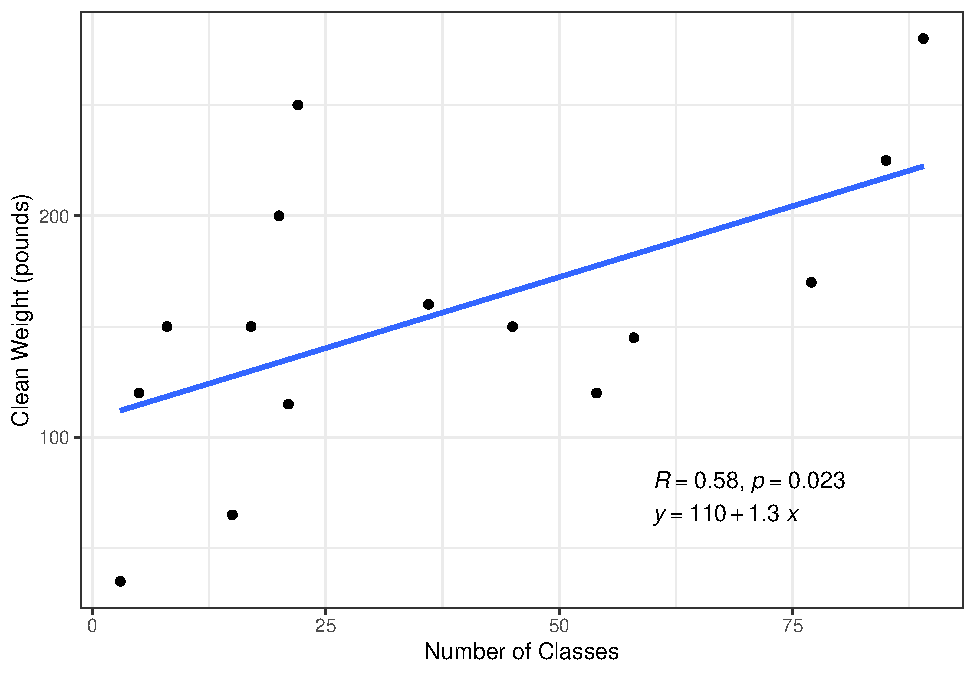
\includegraphics{_main_files/figure-latex/unnamed-chunk-3-1.pdf}

\begin{itemize}
\tightlist
\item
  Our intercept is 110 which can be interpreted as the expected clean weight with 0 classes.
\item
  Our slope is 1.3 which can be interpreted as with each additional crossfit class attended, clean weight will increase by 1.3 pounds on average.
\end{itemize}

Here we'll consider the effects of sex:

\begin{Shaded}
\begin{Highlighting}[]
\FunctionTok{ggplot}\NormalTok{(mydat, }\FunctionTok{aes}\NormalTok{(}\AttributeTok{x=}\NormalTok{classes, }\AttributeTok{y=}\NormalTok{clean\_weight, }\AttributeTok{color=}\NormalTok{sex)) }\SpecialCharTok{+}
  \FunctionTok{geom\_point}\NormalTok{() }\SpecialCharTok{+}
  \FunctionTok{theme\_bw}\NormalTok{() }\SpecialCharTok{+}
  \FunctionTok{labs}\NormalTok{(}\AttributeTok{x =} \StringTok{"Number of Classes"}\NormalTok{, }\AttributeTok{y =} \StringTok{"Clean Weight (pounds)"}\NormalTok{) }\SpecialCharTok{+}
  \FunctionTok{geom\_smooth}\NormalTok{(}\AttributeTok{method =} \StringTok{"lm"}\NormalTok{, }\AttributeTok{se =} \ConstantTok{FALSE}\NormalTok{)  }\SpecialCharTok{+}
  \FunctionTok{stat\_cor}\NormalTok{(}\FunctionTok{aes}\NormalTok{(}\AttributeTok{color =}\NormalTok{ sex), }\AttributeTok{label.x =} \DecValTok{5}\NormalTok{) }\SpecialCharTok{+}
  \FunctionTok{stat\_regline\_equation}\NormalTok{(}\FunctionTok{aes}\NormalTok{(}\AttributeTok{color =}\NormalTok{ sex), }\AttributeTok{label.x =} \DecValTok{35}\NormalTok{) }
\end{Highlighting}
\end{Shaded}

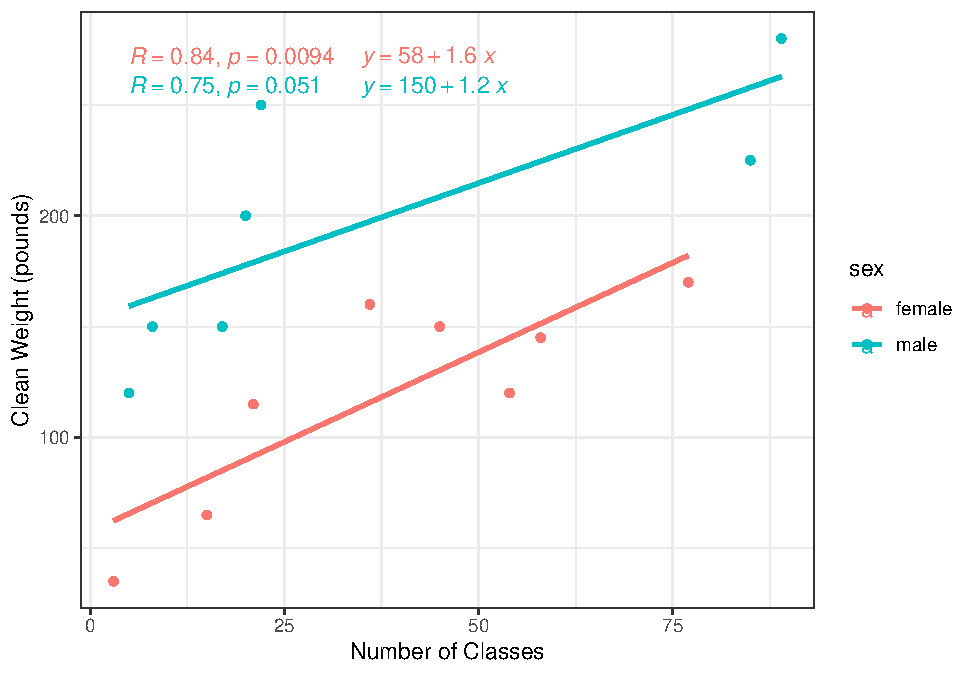
\includegraphics{_main_files/figure-latex/unnamed-chunk-4-1.pdf}

\hypertarget{ordinary-least-sqaures-explained}{%
\section{Ordinary Least Sqaures Explained}\label{ordinary-least-sqaures-explained}}

  \bibliography{book.bib,packages.bib}

\end{document}
